% use paper, or submit
% use 11 pt (preferred), 12 pt, or 10 pt only

%\documentclass[letterpaper, preprint, paper,11pt]{AAS}	% for preprint proceedings
%\documentclass[letterpaper, paper,11pt]{AAS}		% for final proceedings (20-page limit)
%\documentclass[letterpaper, paper,12pt]{AAS}		% for final proceedings (20-page limit)
%\documentclass[letterpaper, paper,10pt]{AAS}		% for final proceedings (20-page limit)
\documentclass[letterpaper, submit]{AAS}			% to submit to JAS

\usepackage{bm}
\usepackage{amsmath}
\usepackage{subfigure}
%\usepackage[notref,notcite]{showkeys}  % use this to temporarily show labels
\usepackage[colorlinks=true, pdfstartview=FitV, linkcolor=black, citecolor= black, urlcolor= black]{hyperref}
\usepackage{overcite}
\usepackage{footnpag}			      	% make footnote symbols restart on each page
\usepackage[outdir=./]{epstopdf}



\PaperNumber{XX-XXX}



\begin{document}

\title{GPS Based Inertial Navigation For Low-Thrust Spacecraft In Cislunar Space}

\author{Grant R. Hecht\thanks{Graduate Student, Department of Mechanical and Aerospace Engineering, University at Buffalo, 240 Bell Hall, Buffalo, NY  14260-4400.}}

\maketitle{} 		

\section{Introduction}
With renewed interest in manned and robotic missions to Earth's moon with the advent of NASA's Artemis Program, robust techniques for navigating spacecraft within cislunar space are necessary. This project will investigate the feasibility of employing pseudorange measurements from the existing GPS satellite constellation alone, as well as with an additional Moon based constellation of navigation satellites, for navigating a low-thrust spacecraft as it spirals towards the target Near-Rectilinear Halo Orbit (NRHO) of the Artemis Lunar Gateway station, starting from a Geostationary Transfer Orbit (GTO) while employing both an Extended and Unscented Kalman Filter. 

\section{Technical Plan}
A feasibility study will be performed to investigate the robustness of GPS based inertial navigation for a spacecraft traversing from a GTO to the NRHO target of the Gateway station. The true GTO to NRHO trajectory has be generated for a low-thrust spacecraft by employing Circular Restricted Three-Body Problem (CR3BP) dynamics, such that fuel use is minimized. An Extended Kalman Filter (EKF) has also been developed, which employs GPS pseudorange and accelerometer measurements, for estimating the inertial states (e.g., position and velocity) and mass of a spacecraft as it travels along the true trajectory. An Unscented Kalman Filter (UKF) will also be developed which estimates the inertial states and mass by employing the same measurements. A simple constellation of Moon orbiting navigation satellites will also be modeled, and the developed EKF and UKF will be modified to ingest pseudorange measurements from the Lunar constellation, in addition to the existing GPS constellation. The performance of both the EKF and UKF, with and without pseudorange measurements from Lunar based navigation satellites, will be analyzed through Monte Carlo analysis.
\subsection{True Trajectory Generation}
The true low-thrust trajectory traversed by the spacecraft has been generated with CR3BP dynamics and a fully continuous, constant specific impulse thrust model by employing the \textit{indirect} approach to optimizing a spacecraft trajectory. Although the details of indirect optimal control are outside of the scope of this project, this category of trajectory optimization methods employ variational calculus and Pontryagin's Maximum Principle to analytically derive the necessary conditions of optimality. This process results in the formation of a two-point boundary value problem (TPBVP) which is solved by finding the set of time varying co-state (adjoint) variables at the initial epoch such that the boundary conditions are satisfied. Details of several techniques used to generate the true trajectory can be found in Reference \citenum{Hecht_2021}.

%For the minimum-fuel trajectory optimization problem, the cost function is given by
%\begin{equation}
%	J = \frac{T_{max}}{c}\int_{t_0}^{t_f}udt
%\end{equation}
%where $T_{max}$ is the maximum thrust available to the spacecraft, $c$ is the exhaust velocity, $u$ is the thrust throttling factor, and $t_i$ and $t_f$ correspond to the initial and final epoch of the trajectory. The TPBVP, while employing CR3BP dynamics, is formulated such that we seek state and co-state trajectories that are a solution of
%\begin{align}
%	\Dot{\mathbf{y}} = \begin{bmatrix} \Dot{\mathbf{x}} \\ 
%	\Dot{\boldsymbol{\lambda}} \end{bmatrix} = \begin{bmatrix} \mathbf{v} \\ 
%	\mathbf{g}(\mathbf{r}) + \mathbf{h}(\mathbf{v}) - \boldsymbol{\lambda}_vuT_{max}/(\lambda_vm) \\ 
%	-uT_{max}/c \\ 
%	-\mathbf{G}^T\boldsymbol{\lambda}_v \\ 
%	-\boldsymbol{\lambda}_r - \mathbf{H}^T\boldsymbol{\lambda}_v \\ 
%	-\lambda_vuT_{max}/m^2
%	\end{bmatrix}
%	\label{eqn:full_ode}
%\end{align}
%while satisfying 
%\begin{equation}
%	\begin{array}{ccc}
%		\mathbf{r}(t_i) - \mathbf{r}_i = 0 & \mathbf{v}(t_i) - \mathbf{v}_i = 0 & m(t_i) - 1 = 0 \\
%		\mathbf{r}(t_f) - \mathbf{r}_f = 0 & \mathbf{v}(t_f) - \mathbf{v}_f = 0 & \lambda_m(t_f) = 0 
%	\end{array}
%\label{eqn:state_cons}
%\end{equation}
%with optimal thrust direction unit vector and throttling factor given by Lawden's primer vector control law (insert citation), where $\mathbf{x} = [\mathbf{r},\mathbf{v},m]^T$ is the $7\times1$ vector of the position, velociy, and mass states, $\boldsymbol{\lambda}=[\boldsymbol{\lambda}_r,\boldsymbol{\lambda_v},\lambda_m]^T$ is the $7\times1$ vector of introduced co-state variables, corresponding to each of the physical states,
%\begin{equation}
%	\mathbf{g}(\mathbf{r}) = \begin{bmatrix}
%	r_x - \frac{(1 - \mu)(r_x + \mu)}{r_1^3} - \frac{\mu(r_x + \mu - 1)}{r_2^3} \\
%	r_y - \frac{(1 - \mu)r_y}{r_1^3} - \frac{\mu r_y}{r_2^3} \\
%	-\frac{(1 - \mu)r_z}{r_1^3} - \frac{\mu r_z}{r_2^3}
%	\end{bmatrix}
%\end{equation}
%\begin{equation}
%	\mathbf{h}(\mathbf{v}) = \begin{bmatrix} 2v_y & -2v_x & 0 \end{bmatrix}^T
%\end{equation}
%\begin{align}
%	r_1 &= \sqrt{(r_x + \mu)^2 + r_y^2 + r_z^2} \\
%	r_2 &= \sqrt{(r_x + \mu - 1)^2 + r_y^2 + r_z^2}
%\end{align}
%and
%\begin{align}
%	\mathbf{G} &= \frac{\partial \mathbf{g}(\mathbf{r})}{\partial \mathbf{r}} \\
%	\mathbf{H} &= \frac{\partial \mathbf{h}(\mathbf{v})}{\partial \mathbf{v}}
%\end{align} 
%
\begin{table}[hbt!]
	\centering
	\caption{Low-Thrust Trajectory Parameters}
	\label{tab:traj_params}
	\begin{tabular}{ccc}
		\hline
		\hline
		Parameter             		 & Value        & Units         \\ 
		\hline
		Initial Mass ($m_0$) 		 & 1500 		& kg            \\
		Exhaust Velocity (c) 		 & 29.43        & km/$\text{s}$  \\
		Specific Impulse ($I_{sp}$)  & 3000  		& s             \\
		Max Thrust ($T_{max}$)       & 10  		 	& N             \\
		Time of Flight ($t_f-t_0$)   & 33.0      	& days          \\
		\hline \hline
	\end{tabular}
\end{table}

By solving the TPBVP derived through indirect optimal control for a spacecraft with parameters shown in Table \ref{tab:traj_params}, the optimal trajectory shown in Figure \ref{fig:traj} was generated, where coasting arcs are shown in blue, thrusting arcs in red, the target NRHO in dashed black lines, and the location of the Earth and Moon as black $\times$ symbols (please note the trajectory is shown in an inertial reference frame and not the CR3BP synodic reference frame).
\begin{figure}[hbt!]
	\centering
	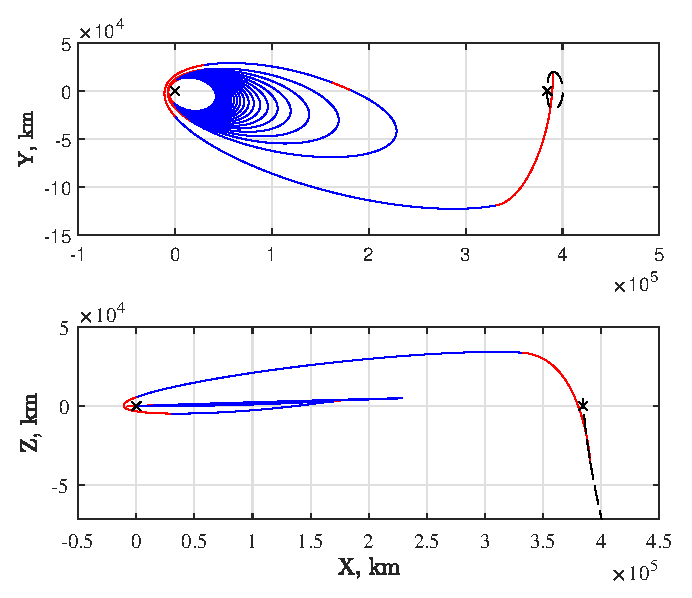
\includegraphics[width=0.6\textwidth]{./../../figures/iTraj.eps}
	\caption{True Low-Thrust Trajectory in Inertial Reference Frame}
	\label{fig:traj}
\end{figure}
As can be seen, the trajectory consists of multiple spirals about the Earth with gradually increasing apogee before finally reaching the NRHO. Therefore, this trajectory should provide a good indication of the developed filters performance in both near Earth and cislunar space.

\subsection{Measurement Modeling}
\subsubsection{GPS Pseudoranges:}
A common GPS pseudorange model is given by \cite{Tapley_2004, Craft_2020}
\begin{align}
	p_{s,k} &= ||\boldsymbol{\rho}_{s/rk,k}|| + c(\Delta t_k - \Delta t_k^s) + \phi_k + \nu_{GPS,k} \\
	\boldsymbol{\rho}_{s/rk,k} &= \mathbf{r}_k^i + \mathbf{T}_b^i\mathbf{r}_{rx}^b - \mathbf{r}_{s,k}^i + \mathbf{T}_{b,s}^i\mathbf{r}_{pc,s}^b
\end{align}
where $p_{s,k}$ is the pseudorange generated from GPS satellite $s$ at time $t_k$, $\Delta t$ is the GNSS receiver clock bias, $\Delta t_k^s$ is the clock bias of GPS satellite $s$, $c$ is the speed of light in a vacuum, $\phi_{s,k}$ is the ionospheric delay, and $\nu_{GPS,k}$ is the receiver white noise. The geometric range is the Euclidean norm of the vector from the phase center of the GPS transmitter and GNSS receiver phase center $\boldsymbol{\rho}_{s/rk,k}$, where $\mathbf{r}_k^i$ is the inertial position of the satellite, $\mathbf{T}_b^i(\bar{\mathbf{q}}_{m,k}) \in SO(3)$ is the rotation from the body frame of the spacecraft to the inertial frame, $\mathbf{r}_{rx}^b$ is the location of the GNSS receiver phase center in the spacecrafts body frame, $\mathbf{r}_{s,k}^i$ is the inertial position of the center of mass of GPS satellite $s$, $\mathbf{T}_{b,s}^i\in SO(3)$ is the rotation from the body frame of GPS satellite $s$ to the inertial frame, and $\mathbf{r}_{pc,s}^b$ is the location of the phase center in the GPS body frame.

For the purposes of this work, we will assume the phase centers of both the GNSS receiver and all GPS transmitters are located at their respective spacecraft's center of mass (i.g., $\mathbf{r}_{rx}^b = \mathbf{r}_{tx}^b = \mathbf{0}_{3\times1}$), thereby decoupling attitude from the pseudorange measurements. We will also assume the GNSS receiver clock is perfect, such that $\Delta t = 0$, and ionospheric effects are negligible. Therefore, our GPS pseudorange model reduces to
\begin{align}
	p_{s,k} &= ||\mathbf{r}_k^i - \mathbf{r}_{s,k}^i|| - c\Delta t_k^s + \nu_{GPS,k}
\end{align}
with relevent partials given by
\begin{equation}
	\frac{\partial p_s}{\partial \mathbf{r}}\bigg|_{\mathbf{x}=\mathbf{x}^*} \approx \frac{\mathbf{r}_k^{i^T} - \mathbf{r}_{s,k}^{i^T}}{||\mathbf{r}_k^i - \mathbf{r}_{s,k}^i||}
\end{equation}
where $(\cdot)^*_k$ is employed to indicated a term associated with the reference trajectory at time $t_k$.

High precision ephemeris data projects provided by IGS \cite{IGSproducts} will be considered as truth and employed to compute the position of GPS satellites at signal transmission times when generating simulated GPS pseudorange measurements. Ephemeris for the Lunar based constellation of navigation satellites will be created by assuming the satellites travel along perfectly circular orbits about the Moon. Perturbed trajectory solutions from the same ephemerides will also be employed when computing expected pseudorange measurements so as to simulate much less precise broadcast ephemeris. IGS ephemeris data products are defined with respect to the Earth fixed IGS14 reference frame, and therefore must be rotated to the Geocentric Celestial Reference Frame (e.g., J200 frame) before they can be employed for inertial navigation. Details of this rotation can be found in Reference \citenum{Vallado_2013}.

\subsubsection{Inertial Measurement Unit}
A highly simplified model of IMU accelerometer measurements will be employed in which accelerometer scale factor error, bias, nonorthoganality, and misalignment are assumed negligible and is given by
\begin{align}
	\mathbf{a}_{IMU,k} = \mathbf{T}_b^{IMU}\mathbf{T}_b^{i^T}\mathbf{a}_k^i + \nu_{IMU,k}
\end{align}
where $\mathbf{a}_k^i$ is the inertial acceleration of the spacecraft at time $t_k$, $\mathbf{T}_b^{IMU}\in SO(3)$ is the rotation from the spacecraft body frame to the IMU frame, and $\nu_{IMU,k}$ is accelerometer white noise. We will also assume the spacecraft body frame and IMU frame are always perfectly aligned with the inertial frame (e.g., $\mathbf{T}_b^{IMU} = \mathbf{T}_b^i = \mathbf{I}_{3\times3}$), thereby allowing the attitde of the spacecraft to be ignored as attitude estimation is outside of the scope of this work. The relevent partials of the accelerometer measurements, assuming perfectly spherical gravitational effects from both the Earth and Moon, are then given by
\begin{align}
	\frac{\partial \mathbf{a}_{IMU}}{\partial \mathbf{r}}\bigg|_{\mathbf{x}=\mathbf{x}^*} &= \frac{\mu}{r^3}\left(\frac{3}{r^2}\mathbf{r}\mathbf{r}^T - \mathbf{I}_{3\times3}\right) + \frac{\mu_l}{r_{ls}^3}\left(\frac{3}{r_{ls}^2}\mathbf{r}_{ls}\mathbf{r}_{ls}^T - \mathbf{I}_{3\times3}\right) \\
	\frac{\partial \mathbf{a}_{IMU}}{\partial m}\bigg|_{\mathbf{x}=\mathbf{x}^*} &= -\frac{u T_{max}}{m^2}\boldsymbol{\alpha}
\end{align}
where $\mathbf{r}_{ls}$ is the vector from the spacecraft to the Moon, $r$ and $r_{ls}$ are the Euclidean norm of $\mathbf{r}$ and $\mathbf{r_{ls}}$ respectively, $\mu$ and $\mu_l$ are the gravitational parameters of the Earth and Moon respectively, $T_{max}$ is the spacecrafts maximum possible thrust, $u$ is the thrust throttling factor, and $\boldsymbol{\alpha}$ is the direction of applied propulsive force.

\section{Preliminary and Expected Results}
Promising preliminary results have already been generated employing the developed EKF with statistical parameters displayed in Table \ref{tab:sim_params}. Accelerometer measurements were processed every 30 seconds, while GPS pseudorange measurements from the existing Earth orbiting GPS constellation were processed every 15 minutes. Figures \ref{fig:posvel_err} and \ref{fig:mass_err} display the filter's error and uncertainty for the inertial and mass states respectively. As can be seen when looking at Figure \ref{fig:posvel_err}, the filter's error is bounded by its realization of the estimation uncertainty $3\sigma$ bounds when estimating all of the inertial states of the spacecraft. Furthermore, the position and velocity of the spacecraft are estimated to within 2 km and 1 m/s for a majority of the transfer from GTO to NRHO, although this is difficult to see when looking at results for the entire 33.1 day trajectory. Finally, we can that estimation error near the NRHO grows slightly due to the increased distance from the GPS satellites, showing the necessity of Lunar navigation satellites if highly accurate navigation is desired. Detailed analysis of estimation performance will be discussed in the final paper. Looking at Figure \ref{fig:mass_err}, we can see that the filter's performance when estimating the mass of the spacecraft is less than ideal. The mass estimate does appear to be biased, and the filter does not properly characterize the mass estimation error uncertainty near the end of the trajectory as the spacecraft approaches the NRHO. This is likely due to the low acceleration due to thrust when compared to gravitational acceleration due to the Earth and Moon, although further analysis is required before this can be said with certainty. 

It is expected that the EKF's estimation accuracy will improve once further tuning of the filter has been performed, and slightly greater performance is expected to be observed for the soon to be developed UKF. Furthermore, the addition of Lunar navigation satellite pseudorange measurements are expected to reduce estimation error when near the Moon, as is the case while approaching the NRHO. Through Monte Carlo analysis, each filter's realization of it's error uncertainty will be compared with the Monte Carlo error statistics to investigate each filter's ability to properly characterize it's uncertainty, and it is expected that the UKF will perform slightly better in this regard due to the use of the unscented transform to propagate uncertainty. The estimation bias and average estimation error of each filter will also be investigated through Monte Carlo analysis.

\begin{table}[]
	\centering
	\caption{Simulation Parameters}
	\label{tab:sim_params}
	\begin{tabular}{ccc}
		\hline
		\hline
		Parameter             		 & Distribution ($1\sigma$) & Units \\ 
		\hline
		GPS Pseudorange Noise 		 & 1 		    & km            	\\
		GPS Broadcase Ephem. Error   & 5            & km  				\\
		Accelerometer Noise          & 10  			& mm/$\text{s}^2$  	\\ 
		\hline
		Initial Position Error       & 0.1  		& km             	\\
		Initial Velocity Error   	 & 10      		& m/s          		\\
		Initial Mass Error 			 & 1			& mg 				\\
		\hline \hline
	\end{tabular}
\end{table}

\begin{figure}[]
	\centering
	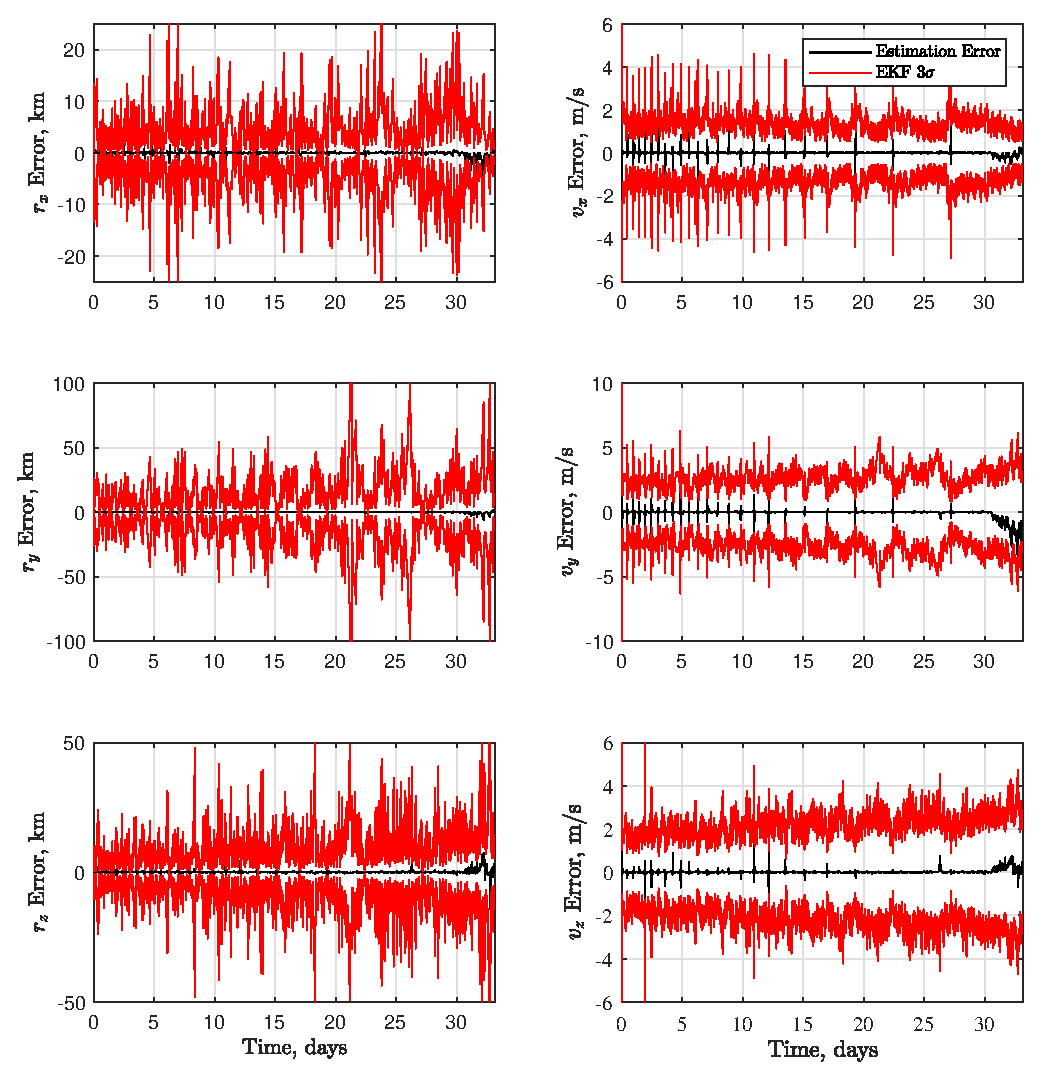
\includegraphics[width=0.8\textwidth]{./../../figures/EKFPosVelError.eps}
	\caption{Position and Velocity Estimation Error and Uncertainty}
	\label{fig:posvel_err}
\end{figure}
\begin{figure}[]
	\centering
	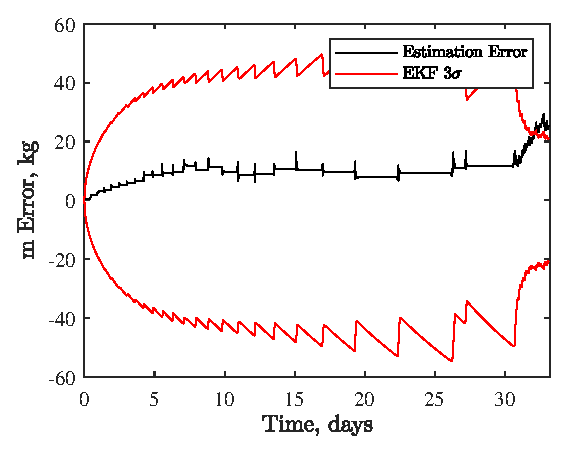
\includegraphics[width=0.4\textwidth]{./../../figures/EKFMass.eps}
	\caption{Mass Estimation Error and Uncertainty}
	\label{fig:mass_err}
\end{figure}


\bibliographystyle{AAS_publication}   % Number the references.
\bibliography{references}   % Use references.bib to resolve the labels.



\end{document}
